\RequirePackage{currfile}
\documentclass[12pt]{beamer}
\usepackage[utf8]{inputenc}
\usepackage[spanish]{babel}
\usepackage{standalone}
\usepackage{color}
\usepackage{siunitx}
\usepackage{hyperref}
%\hypersetup{colorlinks,linkcolor=,urlcolor=blue}
%\hypersetup{colorlinks,urlcolor=blue}
\usepackage{xcolor,soul}
\usepackage{etoolbox}
\usepackage{amsmath}
\usepackage{amsthm}
\usepackage{physics}
\usepackage{multicol}
\usepackage{bookmark}
\usepackage{longtable}
\usepackage{listings}
\usepackage{graphicx}
\usepackage{tikz}
\usetikzlibrary{patterns, matrix, backgrounds, decorations,shapes, arrows.meta}
\usepackage[autostyle,spanish=mexican]{csquotes}
\usepackage[os=win]{menukeys}
\usepackage{pifont}
\usepackage{pbox}
\usepackage{caption}
\captionsetup{font=scriptsize,labelfont=scriptsize}
%\usepackage[sfdefault]{roboto}  %% Option 'sfdefault' only if the base font of the document is to be sans serif

%Sección de definición de colores
\definecolor{ao}{rgb}{0.0, 0.5, 0.0}
\definecolor{bisque}{rgb}{1.0, 0.89, 0.77}
\definecolor{amber}{rgb}{1.0, 0.75, 0.0}
\definecolor{armygreen}{rgb}{0.29, 0.33, 0.13}
\definecolor{alizarin}{rgb}{0.82, 0.1, 0.26}
\definecolor{cadetblue}{rgb}{0.37, 0.62, 0.63}
\definecolor{deepblue}{rgb}{0,0,0.5}
\definecolor{brown}{rgb}{0.59, 0.29, 0.0}
\definecolor{OliveGreen}{rgb}{0,0.25,0}


\usefonttheme[onlymath]{serif}
%Sección de definición de nuevos comandos

\newcommand*{\TitleParbox}[1]{\parbox[c]{1.75cm}{\raggedright #1}}%
\newcommand{\python}{\texttt{python}}
\newcommand{\textoazul}[1]{\textcolor{blue}{#1}}
\newcommand{\azulfuerte}[1]{\textcolor{blue}{\textbf{#1}}}
\newcommand{\funcionazul}[1]{\textcolor{blue}{\textbf{\texttt{#1}}}}
\newcommand{\ptilde}[1]{\ensuremath{{#1}^{\prime}}}
\newcommand{\stilde}[1]{\ensuremath{{#1}^{\prime \prime}}}
\newcommand{\ttilde}[1]{\ensuremath{{#1}^{\prime \prime \prime}}}
\newcommand{\ntilde}[2]{\ensuremath{{#1}^{(#2)}}}
\renewcommand{\arraystretch}{1.5}

\newcounter{saveenumi}
\newcommand{\seti}{\setcounter{saveenumi}{\value{enumi}}}
\newcommand{\conti}{\setcounter{enumi}{\value{saveenumi}}}
\renewcommand{\rmdefault}{cmr}% cmr = Computer Modern Roman

\linespread{1.5}

\usefonttheme{professionalfonts}
%\usefonttheme{serif}
\DeclareGraphicsExtensions{.pdf,.png,.jpg}


%Sección para el tema de beamer, con el theme, usercolortheme y sección de footers
\mode<presentation>
{
  \usetheme{Warsaw}
  \setbeamertemplate{headline}{}
  %\useoutertheme{infolines}
  \useoutertheme{default}
  \usecolortheme{spruce}
  \setbeamercovered{invisible}
  % or whatever (possibly just delete it)
  \setbeamertemplate{section in toc}[sections numbered]
  \setbeamertemplate{subsection in toc}[subsections numbered]
  \setbeamertemplate{subsection in toc}{\leavevmode\leftskip=3.2em\rlap{\hskip-2em\inserttocsectionnumber.\inserttocsubsectionnumber}\inserttocsubsection\par}
  \setbeamercolor{section in toc}{fg=blue}
  \setbeamercolor{subsection in toc}{fg=blue}
  \setbeamercolor{frametitle}{fg=blue}

  \setbeamertemplate{footline}
  %\beamertemplatenavigationsymbolsempty
}

\makeatletter
\setbeamercolor{section in foot}{bg=gray!30, fg=black!90!orange}
\setbeamercolor{subsection in foot}{bg=blue!30!yellow, fg=red}
\setbeamertemplate{footline}
{
  \leavevmode%
  \hbox{%
  \begin{beamercolorbox}[wd=.333333\paperwidth,ht=2.25ex,dp=1ex,center]{section in foot}%
    \usebeamerfont{section in foot} \insertsection
  \end{beamercolorbox}}%
  \begin{beamercolorbox}[wd=.333333\paperwidth,ht=2.25ex,dp=1ex,center]{subsection in foot}%
    \usebeamerfont{subsection in foot}  \insertsubsection
  \end{beamercolorbox}%
  \begin{beamercolorbox}[wd=.333333\paperwidth,ht=2.25ex,dp=1ex,right]{date in head/foot}%
    \usebeamerfont{date in head/foot} \insertshortdate{} \hspace*{2em}
    \insertframenumber{} / \inserttotalframenumber \hspace*{2ex} 
  \end{beamercolorbox}}%
  \vskip0pt%
\makeatother  

\makeatletter
\patchcmd{\beamer@sectionintoc}
  {\vfill}
  {\vskip\itemsep}
  {}
  {}
\makeatother

% \makeatletter
% \patchcmd{\hyper@link@}
%   {{\Hy@tempb}{#4}}
%   {{\Hy@tempb}{\ul{#4}}}
%   {}{}
% \makeatother


% Sección para el código

\definecolor{Code}{rgb}{0,0,0}
\definecolor{Keywords}{rgb}{255,0,0}
\definecolor{Strings}{rgb}{255,0,255}
\definecolor{Comments}{rgb}{0,0,255}
\definecolor{Numbers}{rgb}{255,128,0}

\DeclareCaptionFont{white}{\color{white}}
\DeclareCaptionFormat{listing}{\colorbox{gray}{\parbox{0.99\textwidth}{#1#2#3}}}
\captionsetup[lstlisting]{format=listing,labelfont=white,textfont=white}
\renewcommand{\lstlistingname}{Código}

\lstset{
basicstyle=\ttfamily,
columns=fullflexible,
breaklines=true
}

\lstdefinestyle{codigopython}{%
  language=Python,                % choose the language of the code
  %basicstyle=\footnotesize\small,       % the size of the fonts that are used for the code
  numbers=left,                   % where to put the line-numbers
  numberstyle=\scriptsize,      % the size of the fonts that are used for the line-numbers
  stepnumber=1,                   % the step between two line-numbers. If it is 1 each line will be numbered
  numbersep=5pt,                  % how far the line-numbers are from the code
  backgroundcolor=\color{white},  % choose the background color. You must add \usepackage{color}
  showspaces=false,               % show spaces adding particular underscores
  showstringspaces=false,         % underline spaces within strings
  showtabs=false,                 % show tabs within strings adding particular underscores
  frame=single,   		% adds a frame around the code
  tabsize=2,  		% sets default tabsize to 2 spaces
  captionpos=t,   		% sets the caption-position to bottom
  breaklines=true,    	% sets automatic line breaking
  breakatwhitespace=false,    % sets if automatic breaks should only happen at whitespace
  escapeinside={\#},  % if you want to add a comment within your code
  stringstyle =\color{OliveGreen},
  texcl = true,
  %otherkeywords={{as}},             % Add keywords here
  keywordstyle = \color{blue},
  commentstyle = \color{black},
  identifierstyle = \color{black},
  % literate=%
  %         {á}{{\'a}}1
  %         {é}{{\'e}}1
  %         {í}{{\'i}}1
  %         {ó}{{\'o}}1
  %         {ú}{{\'u}}1
  %
  %keywordstyle=\ttb\color{deepblue}
  %fancyvrb = true,
literate={0}{{\textcolor{red}{0}}}{1}%
            {1}{{\textcolor{red}{1}}}{1}%
            {2}{{\textcolor{red}{2}}}{1}%
            {3}{{\textcolor{red}{3}}}{1}%
            {4}{{\textcolor{red}{4}}}{1}%
            {5}{{\textcolor{red}{5}}}{1}%
            {6}{{\textcolor{red}{6}}}{1}%
            {7}{{\textcolor{red}{7}}}{1}%
            {8}{{\textcolor{red}{8}}}{1}%
            {9}{{\textcolor{red}{9}}}{1}%
            {.0}{{\textcolor{red}{.0}}}{2}% Following is to ensure that only periods
            {.1}{{\textcolor{red}{.1}}}{2}% followed by a digit are changed.
            {.2}{{\textcolor{red}{.2}}}{2}%
            {.3}{{\textcolor{red}{.3}}}{2}%
            {.4}{{\textcolor{red}{.4}}}{2}%
            {.5}{{\textcolor{red}{.5}}}{2}%
            {.6}{{\textcolor{red}{.6}}}{2}%
            {.7}{{\textcolor{red}{.7}}}{2}%
            {.8}{{\textcolor{red}{.8}}}{2}%
            {.9}{{\textcolor{red}{.9}}}{2}%
            {\ }{{ }}{1}% handle the space
        ,%
        %mathescape=true
        %escapeinside={*@}
        escapeinside={A_}{_B}
}

%\usepackage{listings}
\lstset{ %
language=Python,                % choose the language of the code
basicstyle=\small,       % the size of the fonts that are used for the code
numbers=left,                   % where to put the line-numbers
numberstyle=\footnotesize,      % the size of the fonts that are used for the line-numbers
stepnumber=1,                   % the step between two line-numbers. If it is 1 each line will be numbered
numbersep=5pt,                  % how far the line-numbers are from the code
backgroundcolor=\color{white},  % choose the background color. You must add \usepackage{color}
showspaces=false,               % show spaces adding particular underscores
showstringspaces=false,         % underline spaces within strings
showtabs=false,                 % show tabs within strings adding particular underscores
frame=single,   		% adds a frame around the code
tabsize=4,  		% sets default tabsize to 2 spaces
captionpos=b,   		% sets the caption-position to bottom
breaklines=true,    	% sets automatic line breaking
breakatwhitespace=false,    % sets if automatic breaks should only happen at whitespace
escapeinside={\#}{)}          % if you want to add a comment within your code
}

\title{Diferenciación numérica}
\subtitle{Tema 2 - Operaciones matemáticas básicas}
\author[]{M. en C. Gustavo Contreras Mayén}
\date{\today}
%\institute{Facultad de Ciencias - UNAM}
\titlegraphic{
\includegraphics[width=1.75cm]{Imagenes/escudo-facultad-ciencias}\hspace*{4.75cm}~%
   
\includegraphics[width=1.75cm]{Imagenes/escudo-unam}
}
\begin{document}
\maketitle
\fontsize{14}{14}\selectfont
\spanishdecimal{.}
\section*{Contenido}
\frame[allowframebreaks]{\tableofcontents[currentsection, hideallsubsections]}
\section{Introducción}
\frame{\tableofcontents[currentsection, hideothersubsections]}
\subsection{Problema inicial}
\begin{frame}
\frametitle{¿Por qué la diferenciación numérica?}
Sabemos que en la física se pueden modelar sistemas o fenómenos mediante una o un conjunto de ecuación(es) diferencia(les), en donde el manejo tanto de la diferenciación como de la integración serán las estrategias a seguir para obtener una solución de esas ecuaciones.
\end{frame}
\begin{frame}
\frametitle{¿Por qué la diferenciación numérica?}
Suele suceder que la complejidad de las expresiones involucradas no permite un enfoque analítico, aunque el software simbólico moderno nos puede facilitar significativamente la vida como físicos.
\\
\bigskip
Por lo tanto, en muchos casos un tratamiento numérico es inevitable y uno debe estar preparado.
\end{frame}
\begin{frame}
\frametitle{Punto de partida}
Introducimos la noción de diferencias finitas como un concepto básico de la diferenciación numérica.
\\
\bigskip
En un primer momento podremos resolver problemas en donde se presentan derivadas de primer y/o segundo orden, así como el caso de derivadas de varias variables.
\end{frame}
\begin{frame}
\frametitle{Problema inicial}
Consideremos una función dada $f(x)$ en el intervalo finito $[a, b] \in \mathbb{R}$, nos interesa calcular
\begin{align*}
\dv[n]{f(x)}{x}
\end{align*}
\end{frame}
\begin{frame}
\frametitle{Diferenciación numérica}
Usaremos la diferenciación numérica para el siguente problema: se nos da una función $y = f(x)$ y deseamos obtener una de sus derivadas en el punto $x = x_{k}$.
\end{frame}
\begin{frame}
\frametitle{Diferenciación numérica}
Cuando decimos una función \enquote{dada} significa que, o bien tenemos un algoritmo para calcular la función, o contamos con un conjunto de puntos discretos $(x_{i}, y_{i})$, $i = 0, 1,\ldots,N$.
\\
\bigskip
En cualquier caso, tenemos acceso a un número finito de pares de datos $(x, y)$ a partir del cual, podemos calcular la derivada.
\end{frame}
\begin{frame}
\frametitle{Técnica de apoyo para la diferenciación}
Si estás pensando en que la diferenciación numérica se relaciona con interpolación, tienes toda la razón.
\\
\bigskip
Ya que es un medio para encontrar la derivada a partir de una aproximación con un polinomio, y luego diferenciar.
\end{frame}
\begin{frame}
\frametitle{Otra técnica de apoyo}
Una herramienta igualmente eficaz es el desarrollo en serie de Taylor de $f(x)$ sobre el punto de $x_{k}$, lo que representa como ventaja de que nos proporciona información acerca del error cometido en la aproximación.
\end{frame}
\begin{frame}
\frametitle{Limitación de la diferenciación numérica}
La diferenciación numérica \emph{no es un proceso particularmente exacto:} se presenta un conflicto entre los errores de redondeo (debido a la precisión de la máquina) y los errores inherentes a la interpolación.
\\
\bigskip
Por esta razón, la derivada de una función no debe de ser calculada con la misma precisión que la propia función.
\end{frame}
\section{Diferencias finitas}
\frame{\tableofcontents[currentsection, hideothersubsections]}
\subsection{Definición}
\begin{frame}
\frametitle{Definición de diferencias finitas}
De la función suave $f(x)$ en $[a, b] \in \mathbb{R}$, se divide el intervalo en $N - 1$ subintervalos espaciados uniformemente tal que
\begin{align*}
[x_{i}, x_{i+1}] \hspace{0.5cm} \text{donde } \hspace{0.2cm} x_{1} = a, x_{N} = b
\end{align*}
\end{frame}
\begin{frame}
\frametitle{Valor de $x_{i}$}
El valor para el punto $x_{i}$ está dado por
\begin{align*}
x_{i} = a + (i - 1) \, \dfrac{b - a}{N - 1} \hspace{1.5cm} i = 1, 2, \ldots, N
\end{align*}
\end{frame}
\begin{frame}
\frametitle{Uso de la variable \textit{h}}
Incorporamos el valor de $h$, como la distancia entre dos puntos vecinos:
\begin{align*}
h = x_{i-1} - x_{i} = \dfrac{b - a}{N - 1} \hspace{1.5cm} \forall \, i = 1, 2, \ldots, N - 1
\end{align*}
\end{frame}
\begin{frame}
\frametitle{Punto importante}
En aras de una notación más compacta, restringimos nuestra discusión \emph{a puntos que están igualmente espaciados}.
\\
\bigskip
El cambio a puntos que están arbitrariamente espaciados al reemplazar $h$ por $h_{i}$ es directa y deja la discusión esencialmente sin cambios.
\end{frame}
\begin{frame}
\frametitle{Número de puntos $x_{i}$}
Considera que el número de puntos en que se divide el intervalo y por lo tanto, su distancia $h$, debe elegirse de tal manera que la función $f(x)$ pueda ser lo \textcolor{blue}{suficientemente aproximada} por sus valores $f(x_{i})$, como se indica en la siguiente figura:
\end{frame}
\begin{frame}
\frametitle{Espacio entre de los puntos del intervalo}
\begin{figure}[h!]
    \centering
    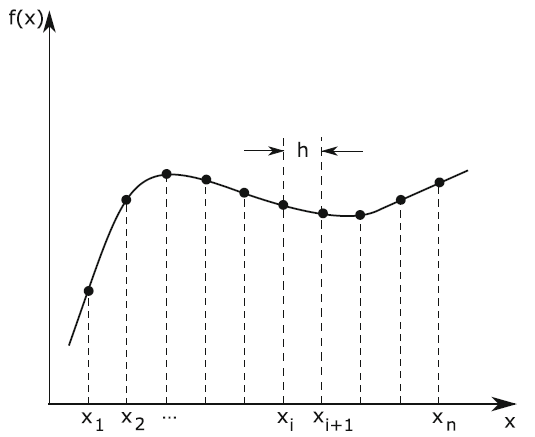
\includegraphics[scale=0.5]{Imagenes/Diferencias_01_Espaciamiento.png}
    \caption{Espaciamiento uniforme de puntos $x_{i}$ en el intervalo.}
    \label{fig:figura_Diferenciacion_01}
\end{figure}
\end{frame}
\begin{frame}
\frametitle{Aproximación por los $x_{i}$}
Entendemos por una  \emph{aproximación suficientemente buena}, aquella que con algún esquema de interpolación en el intervalo $[x_{i}, x_{i+1}]$ reproducirá la función $f(x)$  dentro de la precisión requerida.
\end{frame}
\begin{frame}
\frametitle{Casos especiales}
Se pueden presentar dos casos especiales:
\setbeamercolor{item projected}{bg=blue!70!black,fg=yellow}
\setbeamertemplate{enumerate items}[circle]
\begin{enumerate}[<+->]
\item La función varía mucho dentro de algún subintervalo $[c, d] \in [a, b]$
\item La función varía lentamente dentro de $[a, b] \setminus [c, d]$
\end{enumerate}
\pause
Si esto ocurre, se aconseja utilizar un espaciado variable de puntos, es decir, $h_{i}$ para reducir el costo computacional del procedimiento.
\end{frame}
\subsection{Notación necesaria}
\begin{frame}
\frametitle{Notación necesaria}
Presentamos la siguiente notación: El valor de la función $f(x)$ en el punto $x_{i}$, la escribiremos como $f_{i} \equiv f(x_{i})$, y su derivada de n-ésimo orden es:
\begin{align*}
f_{i}^{(n)} = f^{(n)}(x_{i}) = \dv[n]{f(x)}{x}\eval_{x=x_{i}} 
\end{align*}
\end{frame}
\begin{frame}
\frametitle{Notación necesaria}
Además, definimos para un valor $\xi$ arbitrario tal que $\xi \in [x_{i}, x_{i+1})$
\begin{align*}
f_{i+\varepsilon}^{(n)} = f^{(n)}(\xi)
\end{align*}
\pause
donde $f_{i+\varepsilon}^{(0)} \equiv f_{i+\varepsilon}$, y $\varepsilon$ se escoge para obtener
\begin{align*}
\xi = x_{i} + \varepsilon \, h \hspace{1.5cm} \varepsilon \in [0, 1)
\end{align*}
\end{frame}
\begin{frame}
\frametitle{Primer vistazo a la derivada}
Sabemos del cálculo que la primera derivada $f^{\prime}(x)$ de una función $f(x)$ la cual es suave en el intervalo $[a, b]$, para un punto arbitrario $x \in [a, b]$, se define por alguna de las tres siguientes expresiones:
\end{frame}
\begin{frame}
\frametitle{Primer vistazo a la derivada}
\begin{eqnarray*}
f^{\prime} (x):&=& \lim_{h \to 0} \dfrac{f(x + h) - f(x)}{h} \\[0.5em] \pause
&=& \lim_{h \to 0} \dfrac{f(x) - f(x - h)}{h} \\[0.5em] \pause
&=& \lim_{h \to 0} \dfrac{f(x + h) - f(x - h)}{2 \, h}
\end{eqnarray*}
\end{frame}
\begin{frame}
\frametitle{Problema computacional}
Sin embargo, es imposible manejar numéricamente el límite $h \to 0$, esto se expresa en un error no despreciable debido a la cancelación sustractiva.
\end{frame}
\begin{frame}
\frametitle{Solución al problema}
Este problema se evita cuando utilizamos el Teorema de Taylor: si tenemos una función que es $(n+1)$ veces diferenciable y con derivadas continuas en el intervalo $[a, b]$, entonces la función $f(x)$ se puede expresar en términos de una expansión en series de potencias, alrededor del punto $x_{0} \in [a, b]$, como:
\end{frame}
\begin{frame}
\frametitle{Serie de Taylor}
\begin{align*}
f(x) &= \sum_{k=0}^{n} \dfrac{f^{(n) (x_{0})}}{k!} \, (x - x_{0})^{k} + \dfrac{f^{(n+1)}[\xi (x)]}{(n+1)!} \, (x -x_{0})^{n+1} \\[1em]
&{} \forall \, x \in [a, b]
\end{align*}
donde $\xi(x)$ toma un valor entre $x$ y $x_{0}$
\end{frame}
\begin{frame}
\frametitle{Término de error}
El último término del lado derecho de la igualdad anterior, corresponde al error por truncamiento de la serie de Taylor.
\end{frame}
\subsection*{Desarrollo de términos}
\begin{frame}
\frametitle{Desarrollo de los términos}
Ocupando el desarrollo de Taylor de $f(x)$ vamos a revisar las expresiones para los puntos:
\setbeamercolor{item projected}{bg=blue!70!black,fg=yellow}
\setbeamertemplate{enumerate items}[circle]
\begin{enumerate}[<+->]
\item $f(x + h)$
\item $f(x - h)$
\item $f(x + 2 \, h)$
\item $f(x - 2 \, h)$
\end{enumerate}
\end{frame}
\begin{frame}
\frametitle{Desarrollo de los términos}
Los primeros términos para el desarrollo de $f(x + h)$:
\begin{align}
\begin{aligned}
f(x + h) &= f(x) + h \, \ptilde{f} (x) + \dfrac{h^{2}}{2!} \, \stilde{f} (x) + \\
&+ \dfrac{h^{3}}{3!} \, \ttilde{f} (x) + \dfrac{h^{4}}{4!} \, \ntilde{f}{4} (x) + \ldots
\end{aligned}
\label{eq:ecuacion_diferencias_01}
\end{align}
\end{frame}
\begin{frame}
\frametitle{Desarrollo de los términos}
Los primeros términos para el desarrollo de $f(x - h)$:
\begin{align}
\begin{aligned}
f(x - h) &= f(x) - h \, \ptilde{f} (x) + \dfrac{h^{2}}{2!} \, \stilde{f} (x) + \\
&- \dfrac{h^{3}}{3!} \, \ttilde{f} (x) + \dfrac{h^{4}}{4!} \, \ntilde{f}{4} (x) - \ldots
\end{aligned}
\label{eq:ecuacion_diferencias_02}
\end{align}
cuidado con los signos en el cambio de renglón, recuerda que $(+)(-) = (-)$.
\end{frame}
\begin{frame}
\frametitle{Desarrollo de los términos}
Los primeros términos para el desarrollo de $f(x +  2 \, h)$:
\begin{align}
\begin{aligned}
f(x + 2 \, h) &= f(x) + 2 \, h \, \ptilde{f} (x) + \dfrac{(2 \, h)^{2}}{2!} \, \stilde{f} (x) + \\
&+ \dfrac{(2 \, h)^{3}}{3!} \, \ttilde{f} (x) + \dfrac{(2 \, h)^{4}}{4!} \, \ntilde{f}{4} (x) + \ldots
\end{aligned}
\label{eq:ecuacion_diferencias_03}
\end{align}
\end{frame}
\begin{frame}
\frametitle{Desarrollo de los términos}
Los primeros términos para el desarrollo de $f(x -  2 \, h)$:
\begin{align}
\begin{aligned}
f(x - 2 \, h) &= f(x) - 2 \, h \, \ptilde{f} (x) + \dfrac{(2 \, h)^{2}}{2!} \, \stilde{f} (x) + \\
&- \dfrac{(2 \, h)^{3}}{3!} \, \ttilde{f} (x) + \dfrac{(2 \, h)^{4}}{4!} \, \ntilde{f}{4} (x) + \ldots
\end{aligned}
\label{eq:ecuacion_diferencias_04}
\end{align}
\end{frame}
\subsection*{Suma de las diferencias}
\begin{frame}
\frametitle{Suma de las diferencias}
Ahora procedemos a sumar los términos antes desarrollados, para tener:
\setbeamercolor{item projected}{bg=blue!70!black,fg=yellow}
\setbeamertemplate{enumerate items}[circle]
\begin{enumerate}[<+->]
\item Suma de la ec. (\ref{eq:ecuacion_diferencias_01}) más la ec. (\ref{eq:ecuacion_diferencias_02}): $f(x + h) + f(x - h)$
\item Diferencia de la ec. (\ref{eq:ecuacion_diferencias_01}) menos la ec. (\ref{eq:ecuacion_diferencias_02}): $f(x + h) + f(x - h)$
\item Suma de la ec. (\ref{eq:ecuacion_diferencias_03}) más la ec. (\ref{eq:ecuacion_diferencias_04}): $f(x + 2 \, h) + f(x - 2 \, h)$
\item Diferencia de la ec. (\ref{eq:ecuacion_diferencias_03}) menos la ec. (\ref{eq:ecuacion_diferencias_04}): $f(x + 2 \, h) + f(x - 2\,  h)$
\end{enumerate}
\end{frame}
\begin{frame}
\frametitle{Suma de las diferencias}
Para la suma $f(x + h) + f(x - h)$:
\begin{align}
\begin{aligned}
f(x + h) + f(x - h) &= 2 \, f(x) + h^{2} \, \stilde{f} (x) + \\ 
&+\dfrac{h^{4}}{12} \, \ntilde{f}{4} (x) + \ldots
\end{aligned}
\label{eq:ecuacion_diferencias_1p2}
\end{align}
Vemos que se han cancelado términos con signo contrario.
\end{frame}
\begin{frame}
\frametitle{Suma de las diferencias}
Para la diferencia $f(x + h) - f(x - h)$:
\begin{align}
f(x + h) - f(x - h) = 2 \, h \, \ptilde{f} (x) + \dfrac{h^{3}}{3} \, \ttilde{f} (x) + \ldots
\label{eq:ecuacion_diferencias_1m2}
\end{align}
Nuevamente se cancelan términos con signo contrario.
\end{frame}
\begin{frame}
\frametitle{Suma de las diferencias}
Para la suma $f(x + 2\, h) + f(x - 2\, h)$:
\begin{align}
\begin{aligned}
f(x + 2 \, h) + f(x - 2 \, h) &= 2 \, f(x) + 4 \, h^{2} \, \stilde{f} (x) + \\
&+ \dfrac{4 \, h^{4}}{3} \, \ntilde{f}{4} (x) +\ldots
\end{aligned}
\label{eq:ecuacion_diferencias_3p4}
\end{align}
\end{frame}
\begin{frame}
\frametitle{Suma de las diferencias}
Para la diferencia $f(x + 2\, h) - f(x - 2\, h)$:
\begin{align}
\begin{aligned}
f(x + 2 \, h) - f(x - 2 \, h) &= 4 \, h \, \ptilde{f} (x) + \\
&+ \dfrac{8 \, h^{3}}{3} \, \ttilde{f} (x) + \ldots
\end{aligned}
\label{eq:ecuacion_diferencias_3m4}
\end{align}
\end{frame}
\begin{frame}
\frametitle{Revisa con cuidado}
Toma en cuenta que las sumas contienen solo derivadas pares, mientras que las diferencias tienen sólo las derivadas impares.
\end{frame}
\begin{frame}
\frametitle{Revisa con cuidado}
Las ecuaciones (\ref{eq:ecuacion_diferencias_01}) - (\ref{eq:ecuacion_diferencias_3m4}) pueden verse como ecuaciones simultáneas que pueden resolverse para varias derivadas de $f(x)$.
\end{frame}
\begin{frame}
\frametitle{Revisa con cuidado}
El número de ecuaciones involucradas y el número de términos que aparecen en cada ecuación dependerá del orden de la derivada y del grado de precisión deseado para la solución.
\end{frame}
\section{Aproximación por diferencias}
\frame{\tableofcontents[currentsection, hideothersubsections]}
\subsection{Diferencias centrales}
\begin{frame}
\frametitle{Aproximación por diferencias centrales}
De la ec. (\ref{eq:ecuacion_diferencias_1m2}), despejamos el término $\ptilde{f}(x)$ :
\begin{align*}
\ptilde{f}(x) = \dfrac{f(x + h) - f(x - h)}{2 \, h} - \dfrac{h^{2}}{6} \, \ttilde{f} (x) - \ldots
\end{align*} 
\end{frame}
\begin{frame}
\frametitle{Aproximación por diferencias centrales}
Equivalentemente queda expresada como
\begin{align}
\ptilde{f} (x) = \dfrac{f(x + h) - f(x - h)}{2 \, h} + \order{h^{2}}
\label{eq:ecuacion_5_01}
\end{align}
que es llamada \textcolor{blue}{aproximación por diferencias centrales} de $\ptilde{f}(x)$.
\end{frame}
\begin{frame}
\frametitle{Segunda derivada}
De manera similar, de la ec. (\ref{eq:ecuacion_diferencias_1p2}) la aproximación por diferencias centrales para la segunda derivada $\stilde{f}(x)$ es:
\begin{align*}
\stilde{f} (x) &=  \dfrac{f(x + h)- 2 \,  f(x) + f(x - h)}{h^{2}} + \\
&+ \dfrac{h^{2}}{12} \, \ntilde{f}{4}(x) + \ldots
\end{align*}
\end{frame}
\begin{frame}
\frametitle{Segunda derivada}
Es decir:
\begin{align}
\stilde{f} (x) =  \dfrac{f(x + h) - 2 \, f(x) + f(x - h)}{h^{2}} + \order{h^{2}}
\label{eq:ecuacion_5_02}
\end{align}
\end{frame}
\begin{frame}
\frametitle{Limitación de las diferencias centrales}
Las aproximaciones por diferencias centrales no siempre son útiles.
\\
\bigskip
Por ejemplo, considera la situación en que se da la función en los $n$ puntos discretos $x_{0}, x_{1}, \ldots,x_{n}$.  Dado que las diferencias centrales utilizan valores de la función en cada lado de $x$, no sería posible calcular las derivadas en $x_{0}$ y $x_{n}$.
\end{frame}
\begin{frame}
\frametitle{Extendiendo las diferencias centrales}
Es cierto, que necesitamos una expresión para las diferencias finitas que evalúe la función en un sólo lado de $x$.
\\
\bigskip
Estas expresiones son llamadas aproximaciones por diferencias finitas \textcolor{red}{hacia adelante} y \textcolor{blue}{hacia atrás}.
\end{frame}
\subsection*{Diferencias hacia adelante}
\begin{frame}
\frametitle{Diferencias hacia adelante}
De la ec. (\ref{eq:ecuacion_diferencias_01}) despejamos $\ptilde{f} (x)$, para obtener:
\begin{align*}
\ptilde{f} (x) &= \dfrac{f(x + h) - f(x)}{h} - \dfrac{h}{2} \, \stilde{f} (x) + \\
&- \dfrac{h^{2}}{6} \, \ttilde{f} (x) - \ldots
\end{align*}
\end{frame}
\begin{frame}
\frametitle{Diferencias hacia adelante}
Manteniendo los primeros términos, tenemos la \textcolor{red}{aproximación por diferencias centrales hacia adelante}:
\begin{align}
\ptilde{f} (x) = \dfrac{f(x + h) - f(x)}{h} + \order{h}
\label{eq:ecuacion_5_05}
\end{align}
\end{frame}
\subsection*{Diferencias hacia atrás}
\begin{frame}
\frametitle{Diferencias hacia atrás}
De manera análoga, de la ec. (\ref{eq:ecuacion_diferencias_02}) al despejar $\ptilde{f}(x)$, obtenemos la aproximación por diferencias hacia atrás:
\begin{align}
\ptilde{f}(x) = \dfrac{f(x) - f(x - h)}{h} + \order{h}
\label{eq:ecuacion_5_06}
\end{align}
\end{frame}
\begin{frame}
\frametitle{Diferencias hacia atrás}
Hay que hacer notar que el error es $\order{h}$, no es tan bueno comparado con $\order{h^{2}}$ en la aproximación por diferencias centrales.
\end{frame}
\begin{frame}
\frametitle{Comparación entre las aproximaciones}
Con la idea de contar con un esquema que nos ilustre las aproximaciones mencionadas, en la siguiente figura (\ref{fig:figura_Diferenciacion_02}), veremos la aproximación con respecto a la derivada en un punto $x_{i}$ y con los puntos previo y posterior: $x_{i-1}$ y $x_{i+1}$, respectivamente:
\end{frame}
\begin{frame}
\frametitle{Comparación entre las aproximaciones}
\begin{figure}[h!]
    \centering
    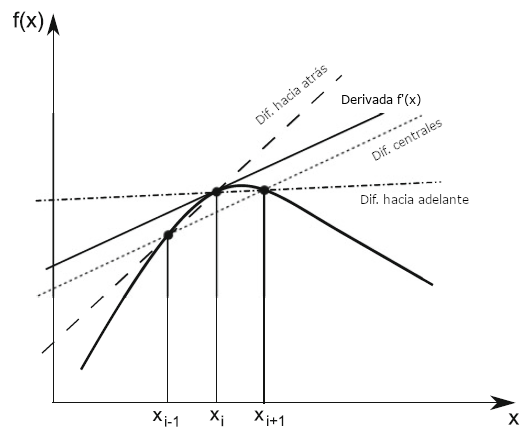
\includegraphics[scale=0.5]{Imagenes/Diferencias_02_Comparacion_Diferencias.png}
    \caption{Comparación entre la derivada $\ptilde{f}(x)$ y las aproximaciones con diferencias finitas.}
    \label{fig:figura_Diferenciacion_02}
\end{figure}
\end{frame}
%Aqui me quedé
\section{Segunda aproximación}
\frame{\tableofcontents[currentsection, hideothersubsections]}
\subsection*{Mejorando la aproximación}
\begin{frame}
\frametitle{Segunda aproximación por diferencias centrales}
Las aproximaciones por diferencias centrales con un error del tipo $\order{h}$ no son tan populares, debido a que es más común usar expresiones con un error del tipo $\order{h^{2}}$.
\end{frame}
\begin{frame}
\frametitle{Segunda aproximación por diferencias centrales}
Para obtener una fórmula con diferencias centrales con este orden de error, tenemos que incluir más términos de la serie de Taylor.
\end{frame}
\subsection*{Expresiones iniciales}
\begin{frame}
\frametitle{Expresiones iniciales}
Consideremos las ecs. (\ref{eq:ecuacion_diferencias_01}) y (\ref{eq:ecuacion_diferencias_03}), para $f(x + h)$ y $f(x + 2 \, h)$, respectivamente.
\\
\bigskip
Eliminamos $\stilde{f}(x)$ multiplicando la ecuación (\ref{eq:ecuacion_diferencias_01}) por $4$ y le restamos la segunda (\ref{eq:ecuacion_diferencias_03}), para obtener:
\end{frame}
\begin{frame}
\frametitle{Expresiones iniciales}
Obtenemos
\begin{align*}
f(x + 2 \, h) - 4 \, f(x + h) &= -3 \, f(x) - 2 \, h \, \ptilde{f}(x) + \\
&+ \dfrac{2 \, h^{3}}{3} \, \ttilde{f}(x) + \ldots
\end{align*}
\end{frame}
\subsection*{Segunda aproximación hacia adelante}
\begin{frame}
\frametitle{Segunda aproximación por diferencias adelante}
Por lo tanto al despejar la primera derivada con respecto a $x$:
\begin{align*}
\ptilde{f}(x) &= \dfrac{-f(x + 2 \, h) + 4 \, f(x + h) + - 3 \, f(x)}{2 \, h} \\
&+ \dfrac{h^{2}}{3} \, \ttilde{f}(x) + \ldots
\end{align*}
\end{frame}
\begin{frame}
\frametitle{Segunda aproximación por diferencias adelante}
Entonces obtenemos la expresión para la \emph{segunda aproximación por diferencias finitas hacia adelante}:
\begin{align}
\ptilde{f}(x) = \dfrac{-f(x + 2 \: h) + 4 \: f(x + h) - 3 \: f(x)}{2 \: h} + \order{h^{2}}
\label{eq:ecuacion_5_08}
\end{align}
\end{frame}
\begin{frame}
\frametitle{Derivadas de orden superior}
La aproximación por diferencias finitas para derivadas de orden superior, involucran términos adicionales de la serie de Taylor.
\\
\bigskip
\pause
Para la aproximación por diferencias hacia adelante para $\stilde{f}(x)$, se deben de incluir los términos $f(x + h)$, $f(x +  2 \, h)$ y $f(x +  3 \, h)$.
\end{frame}
\begin{frame}
\frametitle{Derivadas de orden superior}
La aproximación para $\ttilde{f}(x)$ incluye los términos  $f(x + h)$, $f(x +  2 \, h)$, $f(x +  3 \, h)$ y $f(x +  4 \, h)$, y así sucesivamente.
\\
\bigskip
\pause
Los cálculos para derivadas de orden superior pueden hacerse tediosos.
\end{frame}
\section{Errores en las aproximaciones}
\frame{\tableofcontents[currentsection, hideothersubsections]}
\subsection{Efecto del error}
\begin{frame}
\frametitle{Errores en las aprox. por diferencias finitas}
El efecto del error por redondeo puede ser profundo, si $h$ es muy pequeña, los valores de $f(x)$, $f(x \pm h)$, $f(x \pm 2h)$, etc. serán aproximadamente iguales.
\end{frame}
\begin{frame}
\frametitle{Errores en las aprox. por diferencias finitas}
Cuando se multiplican por los coeficientes y se suman, podemos perder un número grande de términos.
\\
\bigskip
Por otro lado, no debemos de hacer muy grande el valor de $h$, ya que el error debido al truncamiento, sería excesivo.
\end{frame}
\begin{frame}
\frametitle{Propuesta para evitar el error}
Para manejar esta situación que siempre se va a presentar, podemos apoyarnos con el manejo de diferencias finitas en donde se alcance el orden de $\order{h^{2}}$.
\end{frame}
\section{Ejemplos}
\frame{\tableofcontents[currentsection, hideothersubsections]}
\subsection*{Primer Ejemplo}
\begin{frame}
\frametitle{Veamos un ejemplo:}
Queremos calcular la segunda derivada de la función $f(x) = \exp(-x)$ en $x=1$ a partir de la fórmula de diferencias centrales. Varía el valor de $h = 0.64, 0.32, \ldots, 0.00125$.
\\
\bigskip
Calcula el error relativo, considera que el valor exacto es $\stilde{f}(1) = exp(-1) = 0.36787944$, presenta una tabla y discute tus resultados.
\end{frame}
\begin{frame}
\frametitle{Módulo para las aproximaciones}
Dado que ya contamos con las expresiones necesarias para las aproximaciones por diferencias finitas, es conveniente contar dentro de un módulo \funcionazul{ModuloDiferenciacion.py}, el código en \python{} para cada una de las aproximaciones que hemos revisado, de esta manera se podrá utilizar para la solución de los ejercicios.
\end{frame}
\begin{frame}
\frametitle{Resultados obtenidos}
\begin{table}
\centering
\begin{tabular}{c | l | l}
$h$ & Aproximación & Error \\ \hline
$0.64$ & $0.380609096726$ & $3.46028e+00$ \\ \hline
$0.32$ & $0.371029413951$ & $8.56252e-01$ \\ \hline
$0.16$ & $0.368664920656$ & $2.13516e-01$ \\ \hline
$0.08$ & $0.368075685401$ & $5.33450e-02$ \\ \hline
$0.04$ & $0.36792849438$ & $1.33344e-02$ \\ \hline
\end{tabular}
\end{table}
\end{frame}
\begin{frame}
\frametitle{Resultados obtenidos}
\begin{table}
\centering
\begin{tabular}{c | l | l}
$h$ & Aproximación & Error \\ \hline
$0.02$ & $0.367891703983$ & $3.33370e-03$ \\ \hline
$0.01$ & $0.367882506844$ & $8.33655e-04$ \\ \hline
$0.005$ & $0.367880207588$ & $2.08652e-04$ \\ \hline
$0.0025$ & $0.367879632774$ & $5.24015e-05$ \\ \hline
$0.00125$ & $0.36787948904$ & $1.33306e-05$ \\ \hline
\end{tabular}
\end{table}
\end{frame}
\begin{frame}
\frametitle{Resultados de la aproximación}
Vemos que conforme el valor de $h$ disminuye, la aproximación va mejorando y el error relativo va disminuyendo también.
\\
\bigskip
\pause
¿Habrá un momento en donde el error relativo comience a crecer de nuevo debido a que $h$ continúe disminuyendo?
\end{frame}
\subsection*{Segundo Ejemplo}
\begin{frame}
\frametitle{Segundo Ejemplo}
Tenemos un sistema articulado de barras y rótulas con un arreglo que tiene las siguientes dimensiones $a=100$ mm, $b=120$ mm, $c=150$ mm y $d=180$ mm, como podemos ver en la figura:
\end{frame}
\begin{frame}
\frametitle{Segundo Ejemplo}
\begin{figure}[h!]
    \centering
    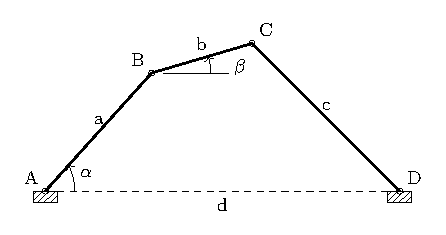
\includegraphics[scale=1.2]{Imagenes/Ejercicio_Diferenciacion_02.eps}
    \caption{Sistema articulado de barras y rótulas.}
\end{figure}
\end{frame}
\begin{frame}
\frametitle{Relación entre los ángulos}
Se puede demostrar a partir de la geometría del problema que la relación entre los ángulos $\alpha$ y $\beta$ es:
\begin{align*}
(d - a \, \cos \alpha &- b \, \cos \beta)^{2} + \\
&+ (a \,  \sin \alpha + b \, \sin \beta)^{2} - c^{2} = 0
\end{align*}
\end{frame}
\begin{frame}
\frametitle{Relación entre los ángulos}
Para un valor dado de $\alpha$, podemos resolver la ecuación para $\beta$, mediante alguno de los métodos para encontrar raíces que ya hemos visto.
\end{frame}
\begin{frame}
\frametitle{Relación entre los ángulos}
Obteniendo el valor de $\beta$ para
\begin{align*}
\alpha=\ang{0}, \ang{5}, \ang{10},\ldots, \ang{30}
\end{align*}
\pause
los resultados son:
\begin{center}
\fontsize{10}{10}\selectfont
\hspace*{-0.5cm}
\begin{tabular}{c | c | c | c | c | c | c | c}
$\alpha$ (grados) & $0$ & $5$ & $10$ & $15$ & $20$ & $25$ & $30$  \\ \hline
$\beta$ (rad) & $1.6595$ & $1.5434$ & $1.4186$ & $1.2925$ & $1.1712$ & $1.0585$ & $0.9561$
\end{tabular}
\end{center}
\end{frame}
\begin{frame}
\frametitle{Problema a resolver}
Si el segmento $AB$ gira con velocidad angular constante de $\SI{25}{\radian\per\second}$, con el método de diferencias finitas de orden $\order{h^{2}}$, calcula la velocidad angular $\dv*{\beta}{t}$ del segmento $BC$ contra el ángulo $\alpha$.
\end{frame}
\begin{frame}
\frametitle{Solución}
La velocidad angular de $BC$ la obtenemos mediante la regla de la cadena:
\begin{align*}
\dv{\beta}{t} = \dv{\beta}{\alpha} \, \dv{\alpha}{t} = 25 \, \dv{\beta}{\alpha} \quad \si{\radian / \second}
\end{align*}
donde $\dv*{\beta}{\alpha}$ se puede estimar con una aproximación de diferencias finitas, tomando los datos de la tabla anterior.
\end{frame}
\begin{frame}
\frametitle{Solución}
Para los puntos extremos se usarían las diferencias hacia adelante y hacia atrás de orden $\order{h^{2}}$, mientras que para los puntos de en medio, el cálculo se hace con las diferencias centrales.
\end{frame}
\begin{frame}
\frametitle{Solución}
Nótese que el incremento del ángulo $\alpha$ en radianes es:
\begin{align*}
h = (\ang{5}) \, \left( \dfrac{\pi}{180} \, \dfrac{\SI{1}{\radian}}{\ang{1}} \right) = \SI{0.087266}{\radian}
\end{align*}
\end{frame}
\begin{frame}
\frametitle{Solución}
Así tenemos que para el primer punto, mediante diferencias finitas de orden $\order{h^{2}}$:
\begin{align*}
\dot{\beta}(\ang{0}) &= 25 \, \dfrac{-3 \, \beta(\ang{0}) + 4 \, \beta(\ang{5}) - \beta(\ang{10})}{2 \, h} = \\
&=  \SI{-32.01}{\radian / \second}
\end{align*}
\end{frame}
\begin{frame}
\frametitle{Solución}
Para los siguientes puntos intermedios, mediante diferencias finitas hacia adelante de orden $\order{h}$:
\begin{align*}
\dot{\beta}(\ang{5}) = \dfrac{\beta(\ang{10}) - \beta(\ang{0})}{2 \, h} = \SI{-34.51}{\radian / \second}
\end{align*}
\end{frame}
\begin{frame}
\frametitle{Para el último punto}
Como queremos que la derivada de $\beta$ sea de orden $\order{h^{2}}$, hay que desarrollar la expresión correspondiente para una segunda aproximación por diferencias hacia atrás.
\\
\bigskip
\pause
\textcolor{red}{Demuestra que esa expresión es}:
\begin{align*}
\ptilde{f}(x) = \dfrac{3 \, f(x) - 4 \, f(x - h) + f(x - 2 \, h)}{2 \, h} + \order{h^{2}}
\end{align*}
\end{frame}
\begin{frame}
\frametitle{Incorporar nuevas funciones en el Módulo}
Contamos con varias funciones en el módulo \funcionazul{ModuloDiferenciacion} que nos permiten evaluar una función $f(x)$ continua.
\\
\bigskip
En este caso, tenemos una serie de puntos discretos, por lo que hay que elaborar nuevas funciones que evalúen la aproximación con el conjunto de puntos, así que hay que elaborarlas e incluirlas debidamente en el módulo.
\end{frame}
\begin{frame}
\frametitle{Ejercicio para entregar: Completa la tabla}
Ya con las nuevas funciones en el \funcionazul{ModuloDiferenciacion}, completa la tabla en una sola ejecución, es decir, no hay que introducir manualmente los datos, sino que sea una tarea autómatizada:
\begin{center}
\fontsize{12}{12}\selectfont
\begin{tabular}{c | c | c | c | c | c | c | c}
$\alpha$ (grados) & $0$ & $5$ & $10$ & $15$ & $20$ & $25$ & $30$  \\ \hline
$\dot{\beta}$ (rad/s) & $-32.01$ & $-34.51$ &  &  &  &  & 
\end{tabular}
\end{center}
\end{frame}
\begin{frame}[fragile]
\frametitle{Resultado obtenido}
El resultado que debes de obtener es el siguiente:
\begin{table}
\centering
\fontsize{12}{12}\selectfont
\begin{tabular}{c | c}
$\alpha$ & $\dot{\beta} \quad [\si{\radian / \second}]$ \\ \hline
$\ang{0}$ & $-32.014017$ \\ \hline
$\ang{5}$ & $-34.506383$ \\ \hline
$\ang{10}$ & $-35.938778$ \\ \hline
$\ang{15}$ & $-35.437440$ \\ \hline
$\ang{20}$ & $-33.518031$ \\ \hline
$\ang{25}$ & $-30.810805$ \\ \hline
$\ang{30}$ & $-27.860073$ \\ \hline
\end{tabular}
\end{table}
\end{frame}
\section{Extrapolación de Richardson}
\frame{\tableofcontents[currentsection, hideothersubsections]}
\subsection{Uso de la técnica}
\begin{frame}
\frametitle{Extrapolación de Richardson}
La Extrapolación de Richardson es un método sencillo para aumentar la precisión de ciertos procedimientos numéricos, incluyendo las aproximaciones por diferencias finitas.
\end{frame}
\begin{frame}
\frametitle{Extrapolación de Richardson}
Supongamos que tenemos la forma de calcular una cantidad $G$.
\\
\bigskip
Por otra parte, si consideramos que el resultado depende de un parámetro $h$, hagamos la aproximación por $g(h)$, tenemos entonces que 
\begin{align*}
G = g(h) + E(h)
\end{align*}
donde $E(h)$ representa el error.
\end{frame}
\begin{frame}
\frametitle{Extrapolación de Richardson}
La extrapolación de Richardson puede remover el error, siempre que tenga la forma $E(h) = c \, h^{p}$, donde $c$ y $p$ son constantes.
\end{frame}
\begin{frame}
\frametitle{Haciendo la operación}
Iniciamos el cálculo para varios valores de $h$, digamos $h = h_{1}$, así
\begin{align*}
G = g(h_{1}) + c \, h_{1}^{p}
\end{align*}
\pause
Repetimos el cálculo con $h = h_{2}$, por tanto:
\begin{align*}
G = g(h_{2}) + c \, h_{2}^{p}
\end{align*}
\end{frame}
\begin{frame}
\frametitle{Fórmula de extrapolación}
Eliminando $c$ y resolviendo para $G$, tenemos que:
\begin{align*}
G = \dfrac{(h_{1}/h_{2})^{p} \, g(h_{2}) - g(h_{1})}{(h_{1}/h_{2})^{p}-1}
\end{align*}
que es la fórmula de Extrapolación de Richardson. 
\end{frame}
\begin{frame}
\frametitle{Fórmula de extrapolación}
En la práctica se usa $h_{2} = h_{1}/2$, quedando:
\begin{align*}
G = \dfrac{2^{p} \, g(h_{1}/2) - g(h_{1})}{2^{p}-1}
\end{align*}
\end{frame}
\subsection*{Ejemplo}
\begin{frame}
\frametitle{Ejemplo}
Usemos el ejemplo de $f(x) = exp(-x)$ y queremos calcular $\stilde{f}(x)$ en $x=1$, consideremos los valores de la tabla:
\begin{table}
\centering
\begin{tabular}{c | l | l}
$h$ & Aproximación & Error \\ \hline
$0.64$ & $0.380609096726$ & $3.46028e+00$ \\ \hline
$0.32$ & $0.371029413951$ & $8.56252e-01$ \\ \hline
$0.16$ & $0.368664920656$ & $2.13516e-01$ \\ \hline
\vdots & & \\ \hline
\end{tabular}
\end{table}
\end{frame}
\begin{frame}
\frametitle{Ejemplo}
Dado que la extrapolación contine errores por truncamiento, debemos limitarnos a los valores de $h$ que producen un redondeo insignificante.
\\
\bigskip
\pause
De la tabla anterior tenemos que:
\begin{align*}
g(0.64) = 0.380609 \hspace{2cm} g(0.32) = 0.371029
\end{align*}
\end{frame}
\begin{frame}
\frametitle{Ejemplo}
El error de truncamiento en la aproximación central por diferencias finitas es:
\begin{align*}
E(h) = \order{h^{2}} = c_{1} \, h^{2} + c_{2} \, h^{4} + c_{3} \, h^{6} + \ldots
\end{align*}
\end{frame}
\begin{frame}
\frametitle{Ejemplo}
Por lo que podemos eliminar el primer término del error (dominante), si usamos $p = 2$ y $h_{1} = 0.64$, así
\begin{align*}
G &= \dfrac{2^{2} \, g(0.32) - g(0.64}{2^{2}-1} = \\[0.5em]
&= \dfrac{4 \, (0.371035) - 0.380610}{3} \\[0.5em]
&= 0.367843
\end{align*}
\end{frame}
\begin{frame}
\frametitle{Mejor aproximación}
Que es una aproximación de $\stilde{f}(x)$ con un error del tipo $\order{h^{4}}$.
\\
\bigskip
\pause
Siendo \emph{el mejor valor obtenido} en comparación de los obtenidos anteriormente.
\end{frame}
\subsection*{Segundo Ejemplo}
\begin{frame}
\frametitle{Segundo Ejemplo}
Teniendo en cuenta el siguiente conjunto de datos uniformemente espaciados:
\begin{table}
\centering
\begin{tabular}{c | c | c | c | c | c }
x & $0$ & $0.1$ & $0.2$ & $0.3$ & $0.4$ \\ \hline
f(x) & $0.0000$ & $0.0819$ & $0.1341$ & $0.1646$ & $0.1797$
\end{tabular}
\end{table}
\end{frame}
\begin{frame}
\frametitle{Segundo Ejemplo}
Calcula $\ptilde{f}(x)$ y $\stilde{f}(x)$ en $x = 0$ y $x = 0.2$, usando la aproximación por diferencias finitas de orden $\order{h^{2}}$.
\end{frame}
\begin{frame}
\frametitle{Solución por diferencias hacia adelante}
Usando la aproximación de orden $\order{h^{2}}$, de la expresión de diferencias finitas hacia adelante, tenemos que:
\begin{eqnarray*}
\ptilde{f}(0) &=& \dfrac{-3 \, f(0) + 4 \, f(0.1) - f(0.2)}{2 \, (0.1)} = 0.967 \\[0.5em]
\pause
\stilde{f}(0) &=& \dfrac{2 \, f(0) - 5 \, f(0.1) + 4 \, f(0.2) - f(0.3)}{(0.1)^{2}} = \\[0.5em]
&=& -3.77
\end{eqnarray*}
\end{frame}
\begin{frame}
\frametitle{Solución por diferencias centrales}
Si usamos ahora la aproximación por diferencias centrales:
\begin{eqnarray*}
\ptilde{f}(0.2) &=& \dfrac{-f(0.1) + f(0.3)}{2 \, (0.1)} = 0.4135 \\[0.5em]
\pause
\stilde{f}(0.2) &=& \dfrac{f(0.1) - 2 \, f(0.2) + f(0.3)}{(0.1)^{2}} = -2.17
\end{eqnarray*}
\end{frame}
\begin{frame}
\frametitle{Problema a resolver}
Usando los datos de la tabla anterior y los valores de $\ptilde{f}(x)$ y $\stilde{f}(x)$, calcular $\ptilde{f}(0)$ con la mayor precisión posible.
\\
\medskip
\pause
Para reportar el valor con la mayor precisión posible, entonces hay que usar el método de extrapolación de Richardson con aproximación de diferencias finitas.
\end{frame}
\begin{frame}
\frametitle{Solución}
Iniciamos con la segunda aproximación por diferencias hacia adelante de orden $\order{h^{2}}$ para $\ptilde{f}(0)$: usamos en una $h = 0.2$ y en otra $h = 0.1$, entonces
\begin{eqnarray*}
g(0.2) &=& \dfrac{-3 \, f(0) + 4 \, f(0.2) - f(0.4)}{2 \, (0.2)} = 0.8918 \\[0.5em]
\pause
g(0.1) &=& \dfrac{-3 \, f(0) + 4 \, f(0.1) - f(0.2)}{2\, (0.1)} = 0.9675
\end{eqnarray*}
\end{frame}
\begin{frame}
\frametitle{Solución}
Recordemos que el error en ambas aproximaciones, es de la forma
\begin{align}
E(h) = c_{1} \, h^{2} + c_{2} \, h^{4} + c_{3} \, h^{5} + \ldots
\end{align}
\end{frame}
\begin{frame}
\frametitle{Solución}
Usamos la extrapolación de Richardson para eliminar el término dominante. Con $p = 2$, resulta
\begin{align*}
\ptilde{f}(0) \simeq G = \dfrac{2^{2} \, g(0.1) - g(0.2)}{2^{2}-1} = 0.9927
\end{align*}
la cual es la mejor aproximación por diferencias finitas, con un orden $\order{h^{4}}$.
\end{frame}
\section{Funciones de varias variables}
\frame{\tableofcontents[currentsection, hideothersubsections]}
\subsection{Caso de dos variables}
\begin{frame}
\frametitle{Punto de partida}
Será de interés la revisión de cómo aproximar derivadas parciales de funciones que dependen de más de una variable.
\\
\bigskip
\pause
Básicamente, esto se puede lograr discretizando independientemente la función de interés en cada variable particular y luego definiendo las derivadas de diferencias finitas correspondientes.
\end{frame}
\begin{frame}
\frametitle{Punto de partida}
Haremos una revisión breve del caso de una función de dos variables.
\\
\bigskip
La extensión a más variables es directa y se sigue de esta primera revisión.
\end{frame}
\begin{frame}
\frametitle{Derivada parcial en dos variables}
Consideramos una función
\begin{align*}
g(x,y) :| (x, y) \in [a, b] \times [c, d]
\end{align*}
\pause
Identifiquemos el espaciamiento en la dirección del eje $x$ por $h_{x}$, mientras que en la dirección del eje $y$, sea $h_{y}$.
\end{frame}
\begin{frame}
\frametitle{Evaluación de las derivadas parciales}
La evaluación de las derivadas de la forma
\begin{align*}
\pdv[n]{g(x,y)}{x} \hspace{1.5cm} \pdv[n]{g(x, y)}{y}
\end{align*}
para un $n$ arbitrario se aproximan con la ayuda de los esquemas presentados anteriormente, sólo se debe tener en cuenta el espaciado en la dirección respectiva.
\end{frame}
\begin{frame}
\frametitle{Derivada mixta}
Revisaremos ahora el caso de la derivada mixta, en particular la de segundo orden:
\begin{align*}
\pdv[2]{g(x, y)}{x}{y}
\end{align*}
Para derivadas de orden mayor, el desarrollo es similar.
\end{frame}
\begin{frame}
\frametitle{Derivada mixta}
Enfocándonos al caso de la derivada por diferencias central, nos gustaría aproximar la derivada en el punto
\begin{align*}
(a + i \, h_{x}, c + j\, h_{y})
\end{align*}
que abreviaremos como $(i, j)$
\end{frame}
\begin{frame}[fragile]
\frametitle{Desarrollo de la derivada mixta}
Tendremos entonces que
\begin{align*}
\pdv{y} \, \pdv{x} \, g(x, y) \eval_{(i,j)} &= \dfrac{1}{2 \, h_{x}} \left[ \pdv{y} g(x, y)\eval_{(i + 1, j)} + \right. \\[0.5em]
&\left. - \pdv{y} g(x, y)\eval_{(i-1, j)} \right] + \order{h_{x}^{2}}
\end{align*}
\end{frame}
\begin{frame}
\frametitle{Desarrollo de la derivada mixta}
\begin{align*}
&= \dfrac{1}{2 \, h_{x}} \left[ \dfrac{g_{i+1, j+1} - g_{i+1, j-1}}{2 \, h_{y}} + \order{h_{y}^{2}} \eval_{(i+1, j)} + \right. \\[0.5em]
&\left. - \dfrac{g_{i-1, j+1} - g_{i-1, j-1}}{2 \, h_{y}} - \order{h_{y}^{2}}\eval_{(i-1, j)}  \right] + \\[0.5em]
&+ \order{h_{x}^{2}}
\end{align*}
en donde $g_{i,j} \equiv g(x_{i}, y_{i})$
\end{frame}
\begin{frame}
\frametitle{Expresión de la derivada mixta}
Cancelando los términos de orden superior:
\begin{align*}
\pdv{y} \, &\pdv{x} g(x, y)\eval_{i ,j} \approx \dfrac{1}{2 \, h_{x}} \, \dfrac{1}{2 \, h_{y}} \times \\[1em]  
&\times g_{i+1, j+1} - g_{i+1, j-1} - g_{i-1, j+1} + g_{i-1, j-1}
\end{align*}
Esta aproximación simple se mejora fácilmente con la ayuda de los métodos desarrollados anteriormente.
\end{frame}
\subsection*{Otros métodos}
\begin{frame}
\frametitle{Otros métodos de aproximación}
Cabe señalar que también hay otros métodos para aproximar las derivadas parciales.
\\
\bigskip
Uno de los métodos más poderosos es el \emph{método de elementos finitos}.
\end{frame}
\begin{frame}
\frametitle{Método del elemento finito}
La diferencia conceptual con el método de diferencias finitas es que uno divide el dominio en subdominios finitos (\emph{elementos}) en lugar de reemplazarlos por conjuntos de puntos de cuadrícula discretos.
\end{frame}
\begin{frame}
\frametitle{Método del elemento finito}
La función de interés, digamos $g(x, y)$, se reemplaza dentro de cada elemento por un polinomio de interpolación.
\\
\bigskip
Sin embargo, este método es bastante complejo y va más allá del alcance de este curso, pero posiblemente lo requieras más adelante en alguna asignatura en particular.
\end{frame}
\begin{frame}
\frametitle{Ejercicio a cuenta}
Considera la función
\begin{align*}
f(x, y) = \cos (x) \, \exp(-y^{2})
\end{align*}
\setbeamercolor{item projected}{bg=blue!70!black,fg=yellow}
\setbeamertemplate{enumerate items}[circle]
\begin{enumerate}[<+->]
\item Calcula numéricamente su gradiente $\grad{f(x, y)}$ y compara con el resultado analítico.
\item Demuestra que numéricamente el gradiente es independiente del rotacional, es decir que 
\begin{align*}
\curl{\grad{f(x, y)}} = 0 \hspace{1.5cm} \forall \, x , y   
\end{align*}
\end{enumerate}
\end{frame}
\end{document}
